Химические формулы и схемы реакций существенно сложнее для автоматической обработки, чем обычный текст, поскольку их естественное представление является не линейной последовательностью символов, а графовой структурой. В молекулярном графе вершины соответствуют атомам, а рёбра — химическим связям; реакция, в свою очередь, может рассматриваться как преобразование одного множества молекулярных графов в другое. Поэтому химическая запись несёт смысл не только через набор символов, но и через топологию, тип связей, ароматичность, заряды, стереохимию и пространственные отношения между фрагментами структуры. Именно это отличает задачу распознавания формул от классического OCR: если для текста ключевой является последовательность символов, то для химической формулы необходимо восстановить структуру графа и затем представить её в форме, пригодной для хранения, поиска и последующего анализа \cite{refTrinajstic,refWarr}.

В органической химии широко используются две распространённые графические нотации представления молекул: подробная (structural formula) и скелетная (line-angle notation)~\cite{refLineAngle} (см. рис.~\ref{fig:comparison_notations}). В подробной записи явно показываются атомы и значительная часть связей, что облегчает интерпретацию человеком, но увеличивает визуальную насыщенность изображения. В скелетной нотации, напротив, большинство атомов углерода и связанные с ними атомы водорода опускаются, а углеродный каркас кодируется линиями, вершины и концы которых интерпретируются как атомы углерода; гетероатомы, кратные связи, заряды и функциональные группы отображаются явно. Именно скелетная запись наиболее типична для органической химии и научных публикаций, однако она значительно усложняет автоматическое распознавание, так как часть информации в ней задаётся по соглашению, а не прописывается явно. В результате алгоритм должен не просто увидеть линии, а восстановить скрытые атомы, валентности и химически допустимую структуру \cite{refWarr}.

 В подробной записи явно показываются атомы и связи между ними, что облегчает интерпретацию человеком, но увеличивает визуальную насыщенность изображения. В скелетной нотации большинство атомов углерода и связанные с ними атомы водорода опускаются, а углеродный каркас кодируется линиями, вершины и концы которых интерпретируются как атомы углерода; гетероатомы, кратные связи, заряды и функциональные группы отображаются явно.

\begin{figure*}[hbtp]
	\centering
	\begin{tabular}{cc}
		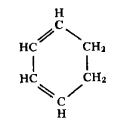
\includegraphics[width=0.25\linewidth]{img/detailed_form.png} & 
		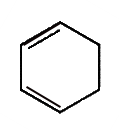
\includegraphics[width=0.25\linewidth]{img/skeletal_form.png} \\
		a$)$ & b$)$	
	\end{tabular}
	\bicaption
	{Пример разных нотаций
		a) подробная; b) скелетная.
	}
	{Example of different notations 
		a) detailed; b) skeletal.	
	}
	\label{fig:comparison_notations}
\end{figure*}

После распознавания графическое изображение молекулы должно быть переведено в машинно-обрабатываемый формат. В современной хемоинформатике для этого используются несколько основных способов представления структур. К числу наиболее распространённых относятся SMILES (Simplified Molecular Input Line Entry System), InChI (International Chemical Identifier), файловые форматы Molfile и SDF, XML-ориентированный CML (Chemical Markup Language), а для реакций — RXNfile, RDF, а также строковые языки наподобие SMIRKS для описания реакционных преобразований. Эти форматы различаются по назначению: одни удобны для компактной линейной записи и поиска, другие — для хранения полной структурной информации, координат, метаданных и реакционных схем. Обзор таких представлений и их роли в химической информатике приведён в работах по компьютерному представлению химических структур и форматам химических данных \cite{refWarr,refDalby,refInChI}.

В данной работе в качестве основного текстового представления структуры выбран формат SMILES, предложенный как компактный язык линейной записи молекул \cite{refWeininger1,refWeininger2}. Его выбор обусловлен несколькими причинами. Во-первых, SMILES является кратким и человекочитаемым: одна молекула кодируется строкой, удобной для хранения в базах данных, индексации, поиска и передачи между программными компонентами. Во-вторых, SMILES широко поддерживается в современных библиотеках и инструментах хемоинформатики, что облегчает интеграцию распознанных структур в конвейер обработки, верификации и поиска. В-третьих, SMILES особенно удобен в задачах, где химическая информация должна быть включена в текстовый или гибридный контур обработки — например, при индексировании документов, построении RAG-систем, текстовом сравнении структур или использовании языковых моделей. В отличие от графического изображения, строка SMILES может быть быстро сопоставлена, нормализована, проверена на корректность и преобразована обратно в молекулярный граф, что делает её практическим компромиссом между компактностью, выразительностью и вычислительной удобностью \cite{refWeininger1,refWarr}.

При этом важным свойством SMILES является неоднозначность представления (см. рис.~\ref{fig:ambiguity_smileys}): одна и та же молекула может быть записана несколькими различными, но эквивалентными строками. Это связано с тем, что линейная запись строится на основе обхода графа, а один и тот же граф допускает разные порядки обхода, разные точки старта, разные способы нумерации циклов, а также различные варианты явного или неявного задания некоторых структурных особенностей. Например, одна и та же структура может быть записана через разные эквивалентные последовательности ветвлений. В задачах хранения и поиска это создаёт проблему: если использовать произвольный SMILES, то идентичные молекулы могут быть представлены разными строками, что затрудняет дедупликацию, построение индексов и сопоставление результатов распознавания \cite{refWeininger2}.

\begin{figure*}[hbtp]
	\centering
	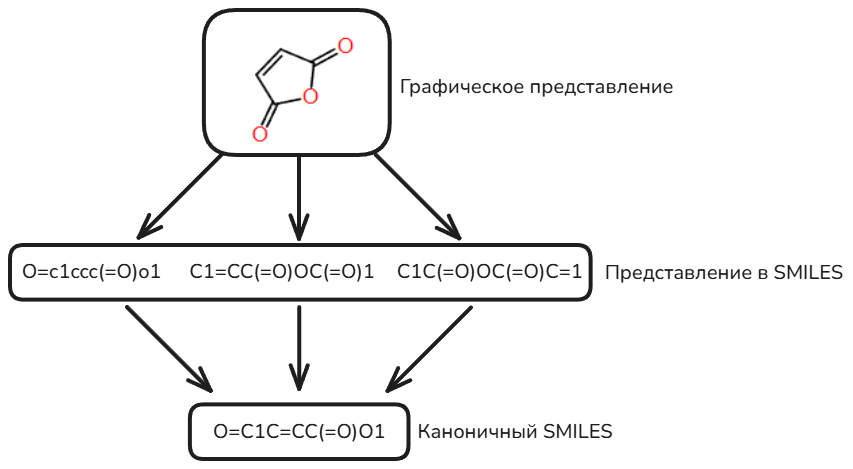
\includegraphics[width=0.75\linewidth]{img/canon_smailes.png}
	\bicaption
	{пример неоднозначного представление форму}
	{example of ambiguous form representation}
	\label{fig:ambiguity_smileys}
\end{figure*}

Для устранения этой неоднозначности используется канонический SMILES, то есть строковое представление, которое строится по детерминированному алгоритму канонизации и назначает данной структуре единственную <<стандартную>> форму записи в рамках конкретной программной системы. Идея канонизации состоит в том, чтобы сначала определить уникальный порядок атомов на основе свойств графа, а затем сгенерировать строку по фиксированным правилам обхода. Это позволяет переводить множество эквивалентных SMILES-представлений одной и той же молекулы к одной нормализованной форме. Однако важно учитывать, что канонический SMILES не является абсолютно универсальным мировым стандартом: разные программные пакеты могут использовать разные алгоритмы канонизации, поэтому канонические строки, полученные, например, в двух различных хемоинформатических библиотеках, могут отличаться при сохранении химической эквивалентности. Тем не менее в рамках одного конвейера обработки канонический SMILES является чрезвычайно полезным инструментом, поскольку обеспечивает нормализацию результатов распознавания, устойчивое сравнение структур и корректную интеграцию извлечённых данных в базы знаний и поисковые индексы \cite{refWeininger2,refOBoyleCanonical,refInChI}. Таким образом, выбор SMILES в сочетании с последующей канонизацией представляет собой практически оправданное решение для задач оцифровки и структурирования химической литературы.

